%%%%%%%%%%%%%%%%%%%%%%%%%%%%%%%%%%%%%%%%%%%%%%%%%%%%%%%%%%%%%%%%%%%%%%%%%%%%%%%%%%
\begin{frame}[fragile]\frametitle{}
\begin{center}
{\Large Model Evaluation with Scikit-Learn}
\end{center}
\end{frame}

%%%%%%%%%%%%%%%%%%%%%%%%%%%%%%%%%%%%%%%%%%%%%%%%%%%%%%%%%%%%%%%%%%%%%%%%%%%%%%%%%%
\begin{frame}[fragile]\frametitle{}
\begin{center}
{\Large Classification Model Evaluation for Pima-Indians Diabetis Dataset}

{\tiny (Ref: Metrics To Evaluate Machine Learning Algorithms in Python - Jason Brownlee)}
\end{center}
\end{frame}

%%%%%%%%%%%%%%%%%%%%%%%%%%%%%%%%%%%%%%%%%%%%%%%%%%%%%%%%%%%
\begin{frame}[fragile]\frametitle{Read Data: the Same Pima Dataset}
Same load step as the preprocessing section, repeated so this section stands on its own.
\begin{lstlisting}
import pandas
import numpy

url = "https://raw.githubusercontent.com/jbrownlee/Datasets/master/pima-indians-diabetes.data.csv"
names = ['preg', 'plas', 'pres', 'skin', 'test', 'mass', 'pedi', 'age', 'class']

dataframe = pandas.read_csv(url, names=names)
array = dataframe.values

# separate array into input and output components
X = array[:,0:8]
y = array[:,8]
\end{lstlisting}
\end{frame}

%%%%%%%%%%%%%%%%%%%%%%%%%%%%%%%%%%%%%%%%%%%%%%%%%%%%%%%%%%%
\begin{frame}[fragile]\frametitle{Classification Accuracy}

	\begin{itemize}
	\item Classification accuracy is the number of correct predictions as a ratio of all predictions made.
	\item This is the most common evaluation metric for classification problems, and also the most misused.
	\item It is only suitable when each class has roughly the same number of observations, which is rarely the case.
	\item It also assumes every kind of prediction error costs the same, which is often untrue.
	\end{itemize}

\end{frame}

%%%%%%%%%%%%%%%%%%%%%%%%%%%%%%%%%%%%%%%%%%%%%%%%%%%%%%%%%%%
\begin{frame}[fragile]\frametitle{Classification Accuracy}
Accuracy score of approximately 77\% accurate
\begin{lstlisting}
from sklearn import model_selection
from sklearn.linear_model import LogisticRegression

seed = 7
kfold = model_selection.KFold(n_splits=10, shuffle=True, random_state=seed)
model = LogisticRegression(max_iter=1000)
scoring = 'accuracy'
results = model_selection.cross_val_score(model, X, y, cv=kfold, scoring=scoring)
print("Accuracy: %.3f (%.3f)" % (results.mean(), results.std()))

# Output:
# Accuracy: 0.772 (0.050)
\end{lstlisting}
\end{frame}



%%%%%%%%%%%%%%%%%%%%%%%%%%%%%%%%%%%%%%%%%%%%%%%%%%%%%%%%%%%
\begin{frame}[fragile]\frametitle{Logarithmic Loss}

	\begin{itemize}
	\item Logarithmic loss (or logloss) is a performance metric for evaluating the predictions of probabilities of membership to a given class.
	\item The scalar probability between 0 and 1 can be seen as a measure of confidence for a prediction by an algorithm. Predictions that are correct or incorrect are rewarded or punished proportionally to the confidence of the prediction.
	\end{itemize}
	
\end{frame}

%%%%%%%%%%%%%%%%%%%%%%%%%%%%%%%%%%%%%%%%%%%%%%%%%%%%%%%%%%%
\begin{frame}[fragile]\frametitle{Logarithmic Loss}
Smaller logloss is better with 0 representing a perfect logloss. As mentioned above, the measure is inverted to be ascending when using the cross\_val\_score() function.
\begin{lstlisting}
seed = 7
kfold = model_selection.KFold(n_splits=10, shuffle=True, random_state=seed)
model = LogisticRegression(max_iter=1000)
scoring = 'neg_log_loss'
results = model_selection.cross_val_score(model, X, y, cv=kfold, scoring=scoring)
print("Logloss: %.3f (%.3f)" % (results.mean(), results.std()))

# Output:
# Logloss: -0.485 (0.057)
\end{lstlisting}
\end{frame}




%%%%%%%%%%%%%%%%%%%%%%%%%%%%%%%%%%%%%%%%%%%%%%%%%%%%%%%%%%%
% Restored from ml_logisticregression_rocauc.tex (Aug 2026): that ~18-frame block was extracted
% out of Session 10 in an earlier pass purely to control that session's length, not for quality
% reasons. This is a curated subset (8 of the 18 frames) giving the intuition build-up the TikZ
% diagram below jumps straight past -- kept here since this file backs both MLCoEP Session 7 and
% the standalone Main_Seminar_ML_DataPrep, so it lands in whichever "ML evaluation" deck is in use.
%%%%%%%%%%%%%%%%%%%%%%%%%%%%%%%%%%%%%%%%%%%%%%%%%%%%%%%%%%%
\begin{frame}[fragile]\frametitle{What is ROC?}

\begin{columns}
\begin{column}[T]{0.5\linewidth}
\begin{itemize}
\item ROC: Receiver Operating Characteristics Curve
\item Tells us how well the model can distinguish between two things (e.g.\ does a patient have a disease or not).
\item Better models accurately distinguish between the two.
\item Predictions are plotted on x, colors show True or False. Y is frequency or count.
\end{itemize}
\end{column}
\begin{column}[T]{0.5\linewidth}
\begin{center}

\includegraphics[width=0.9\linewidth]{roc1}
\end{center}
\tiny{(Ref: Let's learn about AUC ROC Curve! - GreyAtom)}
\end{column}
\end{columns}
\end{frame}

%%%%%%%%%%%%%%%%%%%%%%%%%%%%%%%%%%%%%%%%%%%%%%%%%%%%%%%%%%%%%%%%%%%%%%%%
\begin{frame}[fragile]\frametitle{What is Sensitivity and Specificity?}

\begin{columns}
\begin{column}[T]{0.5\linewidth}
\begin{itemize}
\item Sensitivity $= \frac{TP}{TP + FN}$: of the actual Yes cases, how many did we catch?
\item Specificity $= \frac{TN}{TN + FP}$: of the actual No cases, how many did we clear?
\item Sensitivity, Recall and TPR are three names for the same quantity.
\item Lowering the threshold raises sensitivity but lowers specificity: a trade-off.
\item We plot (1 - Specificity) instead, as in the graph.
\end{itemize}
\end{column}
\begin{column}[T]{0.5\linewidth}
\begin{center}

\includegraphics[width=0.7\linewidth]{roc4}
\end{center}
\tiny{(Ref: Let's learn about AUC ROC Curve! - GreyAtom)}
\end{column}
\end{columns}
\end{frame}

%%%%%%%%%%%%%%%%%%%%%%%%%%%%%%%%%%%%%%%%%%%%%%%%%%%%%%%%%%%%%%%%%%%%%%%%
\begin{frame}[fragile]\frametitle{What is AUC?}

\begin{columns}
\begin{column}[T]{0.5\linewidth}
\begin{itemize}
\item The AUC is the area under the ROC curve.
\item It gives us a good idea of how well the model performs.
\item AUC indicates how well the probabilities from the positive classes are separated from the negative classes.
\end{itemize}
\end{column}
\begin{column}[T]{0.5\linewidth}
\begin{center}

\includegraphics[width=0.8\linewidth]{roc6}
\end{center}
\tiny{(Ref: Let's learn about AUC ROC Curve! - GreyAtom)}
\end{column}
\end{columns}
\end{frame}

%%%%%%%%%%%%%%%%%%%%%%%%%%%%%%%%%%%%%%%%%%%%%%%%%%%%%%%%%%%%%%%%%%%%%%%%
\begin{frame}[fragile]\frametitle{ROC AUC: A Worked Picture}

\begin{columns}
\begin{column}[T]{0.5\linewidth}
\begin{itemize}
\item Often used to evaluate performance of a binary classifier: two possible outcomes, Positive and Negative.
\item This is a histogram where red pixels are positive (got admission!) and blue pixels are negative (did not get admitted).
\item 250 students (pixels here) got admitted and 250 did not.
\item Predicted probabilities are on the x axis. Y axis is the count of students with each ACTUAL outcome.
\end{itemize}
\end{column}
\begin{column}[T]{0.5\linewidth}
\begin{center}

\includegraphics[width=0.9\linewidth]{binclass1}
\end{center}
\tiny{(Ref: ROC Curves and Area Under the Curve (AUC) Explained - Data School)}
\end{column}
\end{columns}
\end{frame}

%%%%%%%%%%%%%%%%%%%%%%%%%%%%%%%%%%%%%%%%%%%%%%%%%%%%%%%%%%%%%%%%%%%%%%%%
\begin{frame}[fragile]\frametitle{ROC AUC: A Well-Separated Classifier}

\begin{columns}
\begin{column}[T]{0.5\linewidth}
\begin{itemize}
\item Where the two colored bell curves barely overlap, the classifier separates the classes well.
\item Only a small band in the middle is ambiguous.
\item A threshold placed in that gap gives high accuracy either way.
\end{itemize}
\end{column}
\begin{column}[T]{0.5\linewidth}
\begin{center}

\includegraphics[width=0.9\linewidth]{binclass3}
\end{center}
\tiny{(Ref: ROC Curves and Area Under the Curve (AUC) Explained - Data School)}
\end{column}
\end{columns}
\end{frame}

%%%%%%%%%%%%%%%%%%%%%%%%%%%%%%%%%%%%%%%%%%%%%%%%%%%%%%%%%%%%%%%%%%%%%%%%
\begin{frame}[fragile]\frametitle{ROC AUC: A Poor Classifier}

\begin{columns}
\begin{column}[T]{0.5\linewidth}
\begin{itemize}
\item If the classifier is not good, there is far more overlap in the middle: many misclassifications.
\item Regardless of where the threshold is placed, accuracy stays bad.
\item The ROC curve shifts away from the top-left corner: more errors, at every threshold.
\end{itemize}
\end{column}
\begin{column}[T]{0.5\linewidth}
\begin{center}

\includegraphics[width=0.9\linewidth]{binclass5}
\end{center}
\tiny{(Ref: ROC Curves and Area Under the Curve (AUC) Explained - Data School)}
\end{column}
\end{columns}
\end{frame}

%%%%%%%%%%%%%%%%%%%%%%%%%%%%%%%%%%%%%%%%%%%%%%%%%%%%%%%%%%%%%%%%%%%%%%%%
\begin{frame}[fragile]\frametitle{ROC AUC: Sweeping All Thresholds}

\begin{columns}
\begin{column}[T]{0.5\linewidth}
\begin{itemize}
\item Plot TPR vs.\ FPR for every possible threshold, not just one.
\item The ROC curve visualizes how far the classifier is from the ideal top-left corner across all thresholds at once.
\item The worst classifier is the diagonal line: 50\%, random chance.
\item To reduce this whole curve to one comparable number, use the Area Under it.
\end{itemize}
\end{column}
\begin{column}[T]{0.5\linewidth}
\begin{center}

\includegraphics[width=0.9\linewidth]{binclass8}
\end{center}
\tiny{(Ref: ROC Curves and Area Under the Curve (AUC) Explained - Data School)}
\end{column}
\end{columns}
\end{frame}

%%%%%%%%%%%%%%%%%%%%%%%%%%%%%%%%%%%%%%%%%%%%%%%%%%%%%%%%%%%%%%%%%%%%%%%%
\begin{frame}[fragile]\frametitle{ROC AUC: Reading the Area}

\begin{columns}
\begin{column}[T]{0.5\linewidth}
\begin{itemize}
\item AUC is the area under the ROC curve, divided by the whole square: e.g.\ 0.8 here.
\item A poor (diagonal-line) classifier has area 0.5. The best possible classifier has area 1.
\item Class balance does not affect the AUC calculation itself.
\item Where exactly to set the threshold is a business decision, made after AUC tells you the model is worth deploying.
\end{itemize}
\end{column}
\begin{column}[T]{0.5\linewidth}
\begin{center}

\includegraphics[width=0.9\linewidth]{binclass9}
\end{center}
\tiny{(Ref: ROC Curves and Area Under the Curve (AUC) Explained - Data School)}
\end{column}
\end{columns}
\end{frame}

%%%%%%%%%%%%%%%%%%%%%%%%%%%%%%%%%%%%%%%%%%%%%%%%%%%%%%%%%%%
\begin{frame}[fragile]\frametitle{Area Under ROC Curve}

\adjustbox{valign=t}{%
\begin{minipage}{0.56\linewidth}%
	\begin{itemize}
	\item Area under ROC Curve (AUC) measures how well a binary classifier separates positive cases from negative cases.
	\item An area of 1.0 is a perfect model, an area of 0.5 is no better than random.
	\item The curve trades off sensitivity (the true positive rate, also called recall) against specificity (the true negative rate).
	\end{itemize}
\end{minipage}%
}%
\hfill%
\adjustbox{valign=t}{%
\begin{minipage}{0.4\linewidth}%
\begin{center}
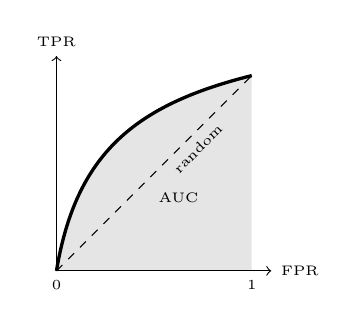
\begin{tikzpicture}[scale=0.62]
\fill[gray!20] (0,0) .. controls (0.4,2.4) and (1.6,3.4) .. (4,4) -- (4,0) -- cycle;
\draw[->] (0,0) -- (4.4,0) node[right,font=\tiny] {FPR};
\draw[->] (0,0) -- (0,4.4) node[above,font=\tiny] {TPR};
\draw[dashed] (0,0) -- (4,4);
\draw[very thick] (0,0) .. controls (0.4,2.4) and (1.6,3.4) .. (4,4);
\node[font=\tiny] at (2.5,1.5) {AUC};
\node[font=\tiny,rotate=45] at (2.9,2.5) {random};
\node[font=\tiny] at (0,-0.3) {0};
\node[font=\tiny] at (4,-0.3) {1};
\end{tikzpicture}
\end{center}
\tiny{The shaded area under the curve is the AUC. The dashed diagonal is a coin-flip model.}
\end{minipage}%
}%

\begin{block}{Intuition}
AUC = 0.5 isn't ``50\% accurate'': it means the model ranks positive and negative cases no better than a coin flip. AUC is threshold-free: it asks how often the model scores a random positive case above a random negative one. That is why it stays meaningful even when the classes are wildly imbalanced, unlike plain accuracy.
\end{block}

\end{frame}

%%%%%%%%%%%%%%%%%%%%%%%%%%%%%%%%%%%%%%%%%%%%%%%%%%%%%%%%%%%
\begin{frame}[fragile]\frametitle{Area Under ROC Curve}
The AUC is relatively close to 1 and greater than 0.5, suggesting some skill in the predictions.
\begin{lstlisting}
seed = 7
kfold = model_selection.KFold(n_splits=10, shuffle=True, random_state=seed)
model = LogisticRegression(max_iter=1000)
scoring = 'roc_auc'
results = model_selection.cross_val_score(model, X, Y, cv=kfold, scoring=scoring)
print("AUC: %.3f (%.3f)" % (results.mean(), results.std()))

# Output:
# AUC: 0.829 (0.047)
\end{lstlisting}
\end{frame}

%%%%%%%%%%%%%%%%%%%%%%%%%%%%%%%%%%%%%%%%%%%%%%%%%%%%%%%%%%%%%%%%%%%%%%%%%%%%%%%%%%
\begin{frame}[fragile]\frametitle{Quick Check: Evaluation Metrics}
\begin{block}{Think About It}
A ``always predict No Cancer'' model that is 99\% accurate on a 99-to-1 imbalanced dataset is useless. What is its AUC, and what does that tell you about which metric to trust here?
\end{block}
\end{frame}

%%%%%%%%%%%%%%%%%%%%%%%%%%%%%%%%%%%%%%%%%%%%%%%%%%%%%%%%%%%%%%%%%%%%%%%%%%%%%%%%%%
\begin{frame}[fragile]\frametitle{Quick Check: Evaluation Metrics}
\begin{block}{Answer}
Its AUC is 0.5, the diagonal, same as random guessing. That model hands every patient the identical score, so it produces no ordering at all, and AUC measures exactly that ordering. Accuracy was flattered by the 99-to-1 class split; AUC was not, because it sweeps every threshold instead of trusting one. On an imbalanced problem, an accuracy near the majority-class share tells you almost nothing: read the confusion matrix and the AUC before believing a model is good.
\end{block}
\end{frame}

%%%%%%%%%%%%%%%%%%%%%%%%%%%%%%%%%%%%%%%%%%%%%%%%%%%%%%%%%%%
% Tier 2, added 2026-08-22: the remaining 8 of the original ~18-frame
% ml_logisticregression_rocauc.tex block (see the "Restored from" comment above this section),
% the mechanical how-to-compute-it half the Aug 2026 curation deliberately left out to keep the
% intuition tier light. Kept as its own block after the Quick Check above rather than interleaved
% into the tier-1 sequence, so an instructor short on time can skip straight to Confusion Matrix.
%%%%%%%%%%%%%%%%%%%%%%%%%%%%%%%%%%%%%%%%%%%%%%%%%%%%%%%%%%%
\begin{frame}[fragile]\frametitle{ROC: Setting a Threshold}

\begin{columns}
\begin{column}[T]{0.5\linewidth}
\begin{itemize}
\item Pick a cutoff value, e.g.\ 0.5, as shown.
\item Positive values above the threshold are correctly predicted: True Positives.
\item Negative values above the threshold are incorrectly predicted as positive: False Positives.
\item Negative values below the threshold are correctly predicted: True Negatives.
\item Positive values below the threshold are incorrectly predicted as negative: False Negatives.
\end{itemize}
\end{column}
\begin{column}[T]{0.5\linewidth}
\begin{center}

\includegraphics[width=0.85\linewidth]{roc2}


\includegraphics[width=0.85\linewidth]{roc3}
\end{center}
\tiny{(Ref: Let's learn about AUC ROC Curve! - GreyAtom)}
\end{column}
\end{columns}
\end{frame}

%%%%%%%%%%%%%%%%%%%%%%%%%%%%%%%%%%%%%%%%%%%%%%%%%%%%%%%%%%%%%%%%%%%%%%%%
\begin{frame}[fragile]\frametitle{Why Plot (1 - Specificity)?}

\begin{columns}
\begin{column}[T]{0.5\linewidth}
\begin{itemize}
\item Specificity is the True Negative Rate.
\item (1 - Specificity) is therefore the False Positive Rate (FPR): the mirror image, looking only at the positives.
\item Raising the threshold lowers both TPR and FPR together. Lowering it raises both together.
\item That is why the ROC curve plots TPR against (1 - Specificity), not Specificity itself: the two move together as the threshold sweeps.
\end{itemize}
\end{column}
\begin{column}[T]{0.5\linewidth}
\begin{center}

\includegraphics[width=0.9\linewidth]{roc7}
\end{center}
\tiny{(Ref: Let's learn about AUC ROC Curve! - GreyAtom)}
\end{column}
\end{columns}
\end{frame}

%%%%%%%%%%%%%%%%%%%%%%%%%%%%%%%%%%%%%%%%%%%%%%%%%%%%%%%%%%%%%%%%%%%%%%%%
\begin{frame}[fragile]\frametitle{ROC AUC: Reading the Histogram}

\begin{columns}
\begin{column}[T]{0.5\linewidth}
\begin{itemize}
\item This is the result of predictions on a validation set, where the actual outcome is also known.
\item Predicted probabilities sit on the x axis. The y axis counts students by their ACTUAL outcome: admitted (red) or not (blue).
\item E.g.\ 10 students were predicted a 0.1 admission probability, and none of them got in: shown as negative (blue).
\end{itemize}
\end{column}
\begin{column}[T]{0.5\linewidth}
\begin{center}

\includegraphics[width=0.9\linewidth]{binclass2}
\end{center}
\tiny{(Ref: ROC Curves and Area Under the Curve (AUC) Explained - Data School)}
\end{column}
\end{columns}
\end{frame}

%%%%%%%%%%%%%%%%%%%%%%%%%%%%%%%%%%%%%%%%%%%%%%%%%%%%%%%%%%%%%%%%%%%%%%%%
\begin{frame}[fragile]\frametitle{ROC AUC: Picking a Threshold at 0.5}

\begin{columns}
\begin{column}[T]{0.5\linewidth}
\begin{itemize}
\item Put the threshold at 0.5: anything above is predicted admitted, anything below is not.
\item With this threshold, accuracy comes out around 90\%.
\item On the ROC curve, this threshold's point sits close to the top-left corner, just short of it due to overlap in the middle of the two histograms.
\end{itemize}
\end{column}
\begin{column}[T]{0.5\linewidth}
\begin{center}

\includegraphics[width=0.9\linewidth]{binclass4}
\end{center}
\tiny{(Ref: ROC Curves and Area Under the Curve (AUC) Explained - Data School)}
\end{column}
\end{columns}
\end{frame}

%%%%%%%%%%%%%%%%%%%%%%%%%%%%%%%%%%%%%%%%%%%%%%%%%%%%%%%%%%%%%%%%%%%%%%%%
\begin{frame}[fragile]\frametitle{ROC AUC: Computing TPR and FPR at 0.8}

\begin{columns}
\begin{column}[T]{0.5\linewidth}
\begin{itemize}
\item TPR: True Positives predicted, divided by all actual positives.
\item FPR: False Positives predicted, divided by all actual negatives.
\item Both range from 0 to 1.
\item At threshold 0.8: TPR is the red pixels to the right of the line (about 50) over all 250 actual positives, so $50/250 = 0.2$.
\item FPR is the blue pixels to the right of the line (0) over all 250 actual negatives, so $0/250 = 0$.
\item That plots one point on the ROC curve, at $x=0$, $y=0.2$.
\end{itemize}
\end{column}
\begin{column}[T]{0.5\linewidth}
\begin{center}

\includegraphics[width=0.9\linewidth]{binclass6}
\end{center}
\tiny{(Ref: ROC Curves and Area Under the Curve (AUC) Explained - Data School)}
\end{column}
\end{columns}
\end{frame}

%%%%%%%%%%%%%%%%%%%%%%%%%%%%%%%%%%%%%%%%%%%%%%%%%%%%%%%%%%%%%%%%%%%%%%%%
\begin{frame}[fragile]\frametitle{ROC AUC: Computing TPR and FPR at 0.5}

\begin{columns}
\begin{column}[T]{0.5\linewidth}
\begin{itemize}
\item At threshold 0.5: TPR is the red pixels to the right of the line (about 230) over 250 actual positives, so $230/250 = 0.94$.
\item FPR is the blue pixels to the right of the line (about 125) over 250 actual negatives, so $125/250 = 0.5$.
\item That plots the next point, at $x=0.5$, $y=0.94$.
\item Repeat at every threshold from 0 to 1 to trace out the full ROC curve.
\end{itemize}
\end{column}
\begin{column}[T]{0.5\linewidth}
\begin{center}

\includegraphics[width=0.9\linewidth]{binclass7}
\end{center}
\tiny{(Ref: ROC Curves and Area Under the Curve (AUC) Explained - Data School)}
\end{column}
\end{columns}
\end{frame}

%%%%%%%%%%%%%%%%%%%%%%%%%%%%%%%%%%%%%%%%%%%%%%%%%%%%%%%%%%%%%%%%%%%%%%%%
\begin{frame}[fragile]\frametitle{ROC AUC: What It Ignores}

\begin{columns}
\begin{column}[T]{0.5\linewidth}
\begin{itemize}
\item AUC depends only on the \emph{order} of the predicted probabilities, not on how confident they are.
\item Two models can rank every example identically, and so produce the same ROC curve and the same AUC, even if one model's probabilities are far better calibrated than the other's.
\item AUC alone cannot tell those two models apart.
\item Log loss can: it penalizes weak or overconfident probabilities directly, not just the ranking.
\end{itemize}
\end{column}
\begin{column}[T]{0.5\linewidth}
\begin{center}

\includegraphics[width=\linewidth]{logreg19}
\end{center}
\tiny{(Ref: Introduction to Data Science - Analytics Vidhya)}
\end{column}
\end{columns}
\end{frame}

%%%%%%%%%%%%%%%%%%%%%%%%%%%%%%%%%%%%%%%%%%%%%%%%%%%%%%%%%%%%%%%%%%%%%%%%
\begin{frame}[fragile]\frametitle{Log Loss}

\begin{columns}
\begin{column}[T]{0.5\linewidth}
\begin{itemize}
\item Adjust the predicted probability for the actual outcome, take its log, then negate it: logs of numbers between 0 and 1 are negative, so the sign flip makes the loss positive.
\item This procedure is what the log-loss formula computes.
\end{itemize}
\begin{block}{Intuition}
Log loss is the penalty for being confidently wrong. Predicting 0.9 for a case that turns out to be 0 costs far more than predicting 0.6 for it, because $-\ln$ of a small number blows up. This is exactly why log loss can separate two models that AUC cannot.
\end{block}
\end{column}
\begin{column}[T]{0.5\linewidth}
\begin{center}

\includegraphics[width=\linewidth]{logreg20}


\includegraphics[width=\linewidth]{logreg21}
\end{center}
\tiny{(Ref: Introduction to Data Science - Analytics Vidhya)}
\end{column}
\end{columns}
\end{frame}

%%%%%%%%%%%%%%%%%%%%%%%%%%%%%%%%%%%%%%%%%%%%%%%%%%%%%%%%%%%
\begin{frame}[fragile]\frametitle{Confusion Matrix}

\adjustbox{valign=t}{%
\begin{minipage}{0.56\linewidth}%
	\begin{itemize}
	\item The confusion matrix presents the accuracy of a model with two or more classes.
	\item Each cell counts how often an actual class was predicted as a given class.
	\item Correct predictions land on the diagonal, every mistake lands off it.
	\item The two mistakes are not the same: a false positive is a false alarm, a false negative is a miss.
	\end{itemize}
\end{minipage}%
}%
\hfill%
\adjustbox{valign=t}{%
\begin{minipage}{0.4\linewidth}%
\begin{center}
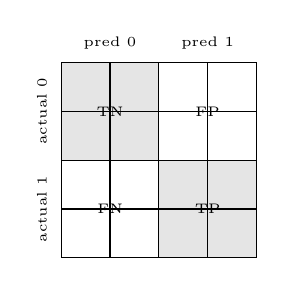
\begin{tikzpicture}[scale=0.62]
\fill[gray!20] (0,2) rectangle (2,4);
\fill[gray!20] (2,0) rectangle (4,2);
\draw (0,0) grid (4,4);
\node[font=\tiny] at (1,3) {TN};
\node[font=\tiny] at (3,3) {FP};
\node[font=\tiny] at (1,1) {FN};
\node[font=\tiny] at (3,1) {TP};
\node[font=\tiny] at (1,4.4) {pred 0};
\node[font=\tiny] at (3,4.4) {pred 1};
\node[font=\tiny,rotate=90] at (-0.4,3) {actual 0};
\node[font=\tiny,rotate=90] at (-0.4,1) {actual 1};
\end{tikzpicture}
\end{center}
\tiny{The shaded diagonal holds the correct predictions. Everything off it is an error.}
\end{minipage}%
}%

\end{frame}

%%%%%%%%%%%%%%%%%%%%%%%%%%%%%%%%%%%%%%%%%%%%%%%%%%%%%%%%%%%
\begin{frame}[fragile]\frametitle{Confusion Matrix}
The majority of the predictions fall on the diagonal line of the matrix (which are correct predictions).
\begin{lstlisting}
from sklearn.metrics import confusion_matrix

test_size = 0.33
seed = 7
X_train, X_test, Y_train, Y_test = model_selection.train_test_split(X, Y, test_size=test_size, random_state=seed)
model = LogisticRegression(max_iter=1000)
model.fit(X_train, Y_train)
predicted = model.predict(X_test)
matrix = confusion_matrix(Y_test, predicted)
print(matrix)

# Output:
# [[142  20]
#  [ 34  58]]
\end{lstlisting}
\end{frame}


%%%%%%%%%%%%%%%%%%%%%%%%%%%%%%%%%%%%%%%%%%%%%%%%%%%%%%%%%%%
\begin{frame}[fragile]\frametitle{Classification Report}

	\begin{itemize}
	\item Scikit-learn does provide a convenience report when working on classification problems to give you a quick idea of the accuracy of a model using a number of measures.
	\item The classification\_report() function displays the precision, recall, f1-score and support for each class.
	\end{itemize}

\end{frame}

%%%%%%%%%%%%%%%%%%%%%%%%%%%%%%%%%%%%%%%%%%%%%%%%%%%%%%%%%%%
\begin{frame}[fragile]\frametitle{Classification Report}
You can see good precision and recall for the algorithm.
\begin{lstlisting}
from sklearn.metrics import classification_report

test_size = 0.33
seed = 7
X_train, X_test, Y_train, Y_test = model_selection.train_test_split(X, Y, test_size=test_size, random_state=seed)
model = LogisticRegression(max_iter=1000)
model.fit(X_train, Y_train)
predicted = model.predict(X_test)
report = classification_report(Y_test, predicted)
print(report)

# Output:
#               precision    recall  f1-score   support
#          0.0       0.81      0.88      0.84       162
#          1.0       0.74      0.63      0.68        92
#     accuracy                           0.79       254
#    macro avg       0.78      0.75      0.76       254
# weighted avg       0.78      0.79      0.78       254
\end{lstlisting}
\end{frame}

%%%%%%%%%%%%%%%%%%%%%%%%%%%%%%%%%%%%%%%%%%%%%%%%%%%%%%%%%%%%%%%%%%%%%%%%%%%%%%%%%%
\begin{frame}[fragile]\frametitle{}
\begin{center}
{\Large Regression Model Evaluation for Boston House Price Dataset}

{\tiny (Ref: Metrics To Evaluate Machine Learning Algorithms in Python - Jason Brownlee)}
\end{center}
\end{frame}

%%%%%%%%%%%%%%%%%%%%%%%%%%%%%%%%%%%%%%%%%%%%%%%%%%%%%%%%%%%
\begin{frame}[fragile]\frametitle{Read Data}
Import Boston House Price dataset and split into Features (X) and target (Y)
\begin{lstlisting}
import pandas

url = "https://raw.githubusercontent.com/jbrownlee/Datasets/master/housing.data"
names = ['CRIM', 'ZN', 'INDUS', 'CHAS', 'NOX', 'RM', 'AGE', 'DIS', 'RAD', 'TAX', 'PTRATIO', 'B', 'LSTAT', 'MEDV']
dataframe = pandas.read_csv(url, sep='\s+', names=names)
array = dataframe.values
X = array[:,0:13]
Y = array[:,13]
\end{lstlisting}
\end{frame}

%%%%%%%%%%%%%%%%%%%%%%%%%%%%%%%%%%%%%%%%%%%%%%%%%%%%%%%%%%%
\begin{frame}[fragile]\frametitle{Mean Absolute Error}

	\begin{itemize}
	\item The Mean Absolute Error (or MAE) is the sum of the absolute differences between predictions and actual values. It gives an idea of how wrong the predictions were.
	\item The measure gives an idea of the magnitude of the error, but no idea of the direction (e.g. over or under predicting).
	\end{itemize}

\end{frame}

%%%%%%%%%%%%%%%%%%%%%%%%%%%%%%%%%%%%%%%%%%%%%%%%%%%%%%%%%%%
\begin{frame}[fragile]\frametitle{Mean Absolute Error}
A value of 0 indicates no error or perfect predictions. Like logloss, this metric is inverted by the cross\_val\_score() function.
\begin{lstlisting}
from sklearn.linear_model import LinearRegression

seed = 7
kfold = model_selection.KFold(n_splits=10, shuffle=True, random_state=seed)
model = LinearRegression()
scoring = 'neg_mean_absolute_error'
results = model_selection.cross_val_score(model, X, Y, cv=kfold, scoring=scoring)
print("MAE: %.3f (%.3f)" % (results.mean(), results.std()))

# Output:
# MAE: -3.387 (0.667)
\end{lstlisting}
\end{frame}


%%%%%%%%%%%%%%%%%%%%%%%%%%%%%%%%%%%%%%%%%%%%%%%%%%%%%%%%%%%
\begin{frame}[fragile]\frametitle{Mean Squared Error}

	\begin{itemize}
	\item The Mean Squared Error (or MSE) is much like the mean absolute error in that it provides a gross idea of the magnitude of error.
	\item Taking the square root of the mean squared error converts the units back to the original units of the output variable and can be meaningful for description and presentation. This is called the Root Mean Squared Error (or RMSE).
	\end{itemize}

\end{frame}

%%%%%%%%%%%%%%%%%%%%%%%%%%%%%%%%%%%%%%%%%%%%%%%%%%%%%%%%%%%
\begin{frame}[fragile]\frametitle{Mean Squared Error}
This metric too is inverted so that the results are increasing. Remember to take the absolute value before taking the square root if you are interested in calculating the RMSE.
\begin{lstlisting}
seed = 7
kfold = model_selection.KFold(n_splits=10, shuffle=True, random_state=seed)
model = LinearRegression()
scoring = 'neg_mean_squared_error'
results = model_selection.cross_val_score(model, X, Y, cv=kfold, scoring=scoring)
print("MSE: %.3f (%.3f)" % (results.mean(), results.std()))

# Output:
# MSE: -23.747 (11.143)
\end{lstlisting}
\end{frame}


%%%%%%%%%%%%%%%%%%%%%%%%%%%%%%%%%%%%%%%%%%%%%%%%%%%%%%%%%%%
\begin{frame}[fragile]\frametitle{$R^2$ Metric}

	\begin{itemize}
	\item The $R^2$ (or R Squared) metric provides an indication of the goodness of fit of a set of predictions to the actual values. In statistical literature, this measure is called the coefficient of determination.
	\item $R^2 = 1$ is a perfect fit, and $R^2 = 0$ means the model does no better than always predicting the mean.
	\item $R^2$ is \emph{not} bounded below by 0: a model that fits worse than that mean-only baseline scores negative, which happens easily on an unrepresentative fold.
	\end{itemize}

\end{frame}

%%%%%%%%%%%%%%%%%%%%%%%%%%%%%%%%%%%%%%%%%%%%%%%%%%%%%%%%%%%
\begin{frame}[fragile]\frametitle{$R^2$ Metric}
Unlike MAE and MSE above, \texttt{'r2'} is not negated by \texttt{cross\_val\_score()}: higher is
already better, so this mean can be read directly. Note \texttt{shuffle=True} in the \texttt{KFold}
below. This dataset is stored in a sorted order, so without shuffling the folds are unrepresentative,
and the score collapses towards the negative-$R^2$ case from the previous slide.
\begin{lstlisting}
seed = 7
kfold = model_selection.KFold(n_splits=10, shuffle=True, random_state=seed)
model = LinearRegression()
scoring = 'r2'
results = model_selection.cross_val_score(model, X, Y, cv=kfold, scoring=scoring)
print("R^2: %.3f (%.3f)" % (results.mean(), results.std()))

# Output:
# R^2: 0.718 (0.099)
\end{lstlisting}
\end{frame}

%%%%%%%%%%%%%%%%%%%%%%%%%%%%%%%%%%%%%%%%%%%%%%%%%%%
\begin{frame}[fragile]\frametitle{Quick Check: Model Evaluation}
\begin{block}{Think About It}
The Pima diabetes dataset has roughly twice as many non-diabetic (class 0) cases as diabetic (class 1) cases. A model that always predicts class 0, no matter the input, could reach around 65\% classification accuracy. Which of the metrics on the earlier slides would immediately expose this model as useless, and why does plain accuracy fail to?
\end{block}
\end{frame}

%%%%%%%%%%%%%%%%%%%%%%%%%%%%%%%%%%%%%%%%%%%%%%%%%%%%%%%%%%%%%%%%%%%%%%%%%%%%%%%%%%
\begin{frame}[fragile]\frametitle{Quick Check: Model Evaluation}
\begin{block}{Answer}
AUC would immediately expose it: a constant-output model can't rank any example above another, so it scores AUC $\approx$ 0.5, no better than random, regardless of class imbalance. The confusion matrix would show the same story directly: an entire empty row or column, since class 1 is never predicted. Accuracy fails here because it only counts how many predictions matched, and on an imbalanced dataset ``always predict the majority class'' matches a lot of the time by construction: exactly why accuracy is called out on the first slide of this section as ``the most misused'' metric.
\end{block}
\end{frame}

%%%%%%%%%%%%%%%%%%%%%%%%%%%%%%%%%%%%%%%%%%%%%%%%%%%
\begin{frame}[fragile]\frametitle{Quick Check: Regression Metrics}
\begin{block}{Think About It}
Two house-price models are each wrong by a total of 10 lakh rupees across 10 houses. Model A is off by 1 lakh on every house. Model B is perfect on 9 houses and off by 10 lakh on the tenth. They have the same MAE. Which model does MSE prefer, and which would you rather deploy?
\end{block}
\end{frame}

%%%%%%%%%%%%%%%%%%%%%%%%%%%%%%%%%%%%%%%%%%%%%%%%%%%%%%%%%%%%%%%%%%%%%%%%%%%%%%%%%%
\begin{frame}[fragile]\frametitle{Quick Check: Regression Metrics}
\begin{block}{Answer}
MSE strongly prefers Model A. Squaring the errors makes one large mistake cost far more than many small ones: Model A scores $10 \times 1^2 / 10 = 1$, while Model B scores $100 / 10 = 10$, ten times worse, even though MAE rates them identically. Which model you deploy depends on the cost of being wrong. If one badly mispriced house is a disaster, use MSE and pick A. If all errors cost the same per rupee, MAE is the honest metric and the two really are equivalent. This is why the two are reported together rather than one replacing the other.
\end{block}
\end{frame}

